\documentclass[sigconf]{acmart}

%%
%% \BibTeX command to typeset BibTeX logo in the docs
\AtBeginDocument{%
  \providecommand\BibTeX{{%
    \normalfont B\kern-0.5em{\scshape i\kern-0.25em b}\kern-0.8em\TeX}}}

%% Rights management information.  This information is sent to you
%% when you complete the rights form.  These commands have SAMPLE
%% values in them; it is your responsibility as an author to replace
%% the commands and values with those provided to you when you
%% complete the rights form.
\setcopyright{acmcopyright}
\copyrightyear{2023}
\acmYear{2023}
\acmDOI{XXXXXXX.XXXXXXX}

%% These commands are for a PROCEEDINGS abstract or paper.
\acmConference[Conference acronym 'XX]{Make sure to enter the correct
  conference title from your rights confirmation emai}{June 03--05,
  2018}{Woodstock, NY}
\acmPrice{15.00}
\acmISBN{978-1-4503-XXXX-X/18/06}


%%
%% Submission ID.
%% Use this when submitting an article to a sponsored event. You'll
%% receive a unique submission ID from the organizers
%% of the event, and this ID should be used as the parameter to this command.
%%\acmSubmissionID{123-A56-BU3}

%%
%% For managing citations, it is recommended to use bibliography
%% files in BibTeX format.
%%
%% You can then either use BibTeX with the ACM-Reference-Format style,
%% or BibLaTeX with the acmnumeric or acmauthoryear sytles, that include
%% support for advanced citation of software artefact from the
%% biblatex-software package, also separately available on CTAN.
%%
%% Look at the sample-*-biblatex.tex files for templates showcasing
%% the biblatex styles.
%%

%%
%% The majority of ACM publications use numbered citations and
%% references.  The command \citestyle{authoryear} switches to the
%% "author year" style.
%%
%% If you are preparing content for an event
%% sponsored by ACM SIGGRAPH, you must use the "author year" style of
%% citations and references.
%% Uncommenting
%% the next command will enable that style.
%%\citestyle{acmauthoryear}

%%
%% end of the preamble, start of the body of the document source.
\begin{document}

%%
%% The "title" command has an optional parameter,
%% allowing the author to define a "short title" to be used in page headers.
\title{Dependability Analysis - Apache commons-imaging library}

%%
%% The "author" command and its associated commands are used to define
%% the authors and their affiliations.
%% Of note is the shared affiliation of the first two authors, and the
%% "authornote" and "authornotemark" commands
%% used to denote shared contribution to the research.
\author{Julian Alexis Orcinoli}
\authornote{All authors contributed equally to this research.}
\affiliation{%
  \institution{Università degli Studi di Salerno}
  \city{Fisciano}
  \state{Salerno}
  \country{Italy}
  \postcode{84084}
}
\email{j.orcinoli@studenti.unisa.it}

\author{Santiago Morales Henao}
\authornote{All authors contributed equally to this research.}
\affiliation{%
  \institution{Università degli Studi di Salerno}
  \city{Fisciano}
  \state{Salerno}
  \country{Italy}
  \postcode{84084}
}
\email{s.moraleshenao@studenti.unisa.it}

\author{Franco Nicolás Merenda}
\authornote{All authors contributed equally to this research.}
\affiliation{%
  \institution{Università degli Studi di Salerno}
  \city{Fisciano}
  \state{Salerno}
  \country{Italy}
  \postcode{84084}
}
\email{f.merenda2@studenti.unisa.it}


%%
%% By default, the full list of authors will be used in the page
%% headers. Often, this list is too long, and will overlap
%% other information printed in the page headers. This command allows
%% the author to define a more concise list
%% of authors' names for this purpose.
\renewcommand{\shortauthors}{Julian A. Orcinoli, Merenda F. Nicolas, and Santiago M. Henao}

%%
%% The abstract is a short summary of the work to be presented in the
%% article.
\begin{abstract}
  This paper presents a comprehensive analysis of software dependability in the context of the Apache Commons Imaging project, a vital component of the Apache Commons IO ecosystem. The study employs a multifaceted approach, leveraging software analytics, testing tools, and vulnerability assessment techniques to evaluate and enhance the dependability and code quality of the project.

  The analysis begins with an exploration of SonarCloud, delving into the identification and resolution of bugs. Subsequently, various software testing tools, including JaCoCo, CodeCov, PiTest, EvoSuite, and Randoop, are employed to assess code coverage, mutation testing, and automated test case generation. The study extends to vulnerability checking using OWASP Dependability Checker and FindSecBugs.
  
  Results showcase improvements in code quality, increased code coverage, and the identification and remediation of software vulnerabilities. The paper contributes valuable insights into the efficacy of diverse tools and methodologies in ensuring software dependability. Through this investigation, we aim to provide a nuanced understanding of the strengths and limitations of each approach, offering guidance for future endeavors in the pursuit of reliable and robust software systems.
\end{abstract}

%%
%% The code below is generated by the tool at http://dl.acm.org/ccs.cfm.
%% Please copy and paste the code instead of the example below.
%%
\begin{CCSXML}
<ccs2012>
   <concept>
       <concept_id>10011007.10011074.10011099.10011102.10011103</concept_id>
       <concept_desc>Software and its engineering~Software testing and debugging</concept_desc>
       <concept_significance>500</concept_significance>
    </concept>
    <concept>
       <concept_id>10011007.10011006.10011073</concept_id>
       <concept_desc>Software and its engineering~Software maintenance tools</concept_desc>
       <concept_significance>500</concept_significance>
   </concept>
   <concept>
       <concept_id>10011007.10011074.10011134.10003559</concept_id>
       <concept_desc>Software and its engineering~Open source model</concept_desc>
       <concept_significance>300</concept_significance>
   </concept>

 </ccs2012>
\end{CCSXML}

\ccsdesc[500]{Software and its engineering~Software testing and debugging}
\ccsdesc[500]{Software and its engineering~Software maintenance tools}
\ccsdesc[300]{Software and its engineering~Open source model}


%%
%% Keywords. The author(s) should pick words that accurately describe
%% the work being presented. Separate the keywords with commas.
\keywords{Software Dependability, Apache Commons Imaging, Software Analytics, SonarCloud, Software Testing Tools, Code Coverage, JaCoCo, CodeCov, Mutation Testing, PiTest, Java Microbenchmark Harness, JMH,  Automated Test Case Generation, EvoSuite, Randoop, Software Vulnerabilities, OWASP Dependability Checker, FindSecBugs, Bug Fixing, Code Quality, Software Engineering}

%% \received{20 February 2007}
%% \received[revised]{12 March 2009}
%% \received[accepted]{5 June 2009}

%%
%% This command processes the author and affiliation and title
%% information and builds the first part of the formatted document.
\maketitle

\section{Introduction}
The concept of software dependability, integral to the fabric of modern computing, has evolved dramatically, underscored by a rich history and the development of complex, multifaceted principles. This journey begins in the era of early mainframes, marked by the efforts to enhance the reliability of these machines for crucial calculations in business and scientific fields. F.P. Brooks Jr., in his seminal work "The Mythical Man-Month," highlighted the inherent complexities in software development, setting the stage for the future discourse on software dependability [1].

As computing systems evolved from monolithic mainframes to interconnected networks, the focus on software dependability widened to encompass not only reliability but also fault tolerance, security, and safety. The 1980s, marked by the introduction of distributed systems, brought forth new challenges in ensuring the dependability of interconnected software systems. R.E. Lyons and W. Vanderkulk, in their pioneering work, emphasized the importance of using redundancy techniques, like Triple-Modular Redundancy, to improve the reliability of these systems [2]. For example, in critical applications like aviation control systems, the implementation of such redundancy techniques ensured uninterrupted operation even in the face of hardware failures.

In the 1990s, with the increasing dependence on software for critical infrastructure and sensitive data management, the focus shifted towards security and safety. D. Gollmann's work on computer security provided foundational insights into protecting software systems in an interconnected world, addressing threats such as unauthorized data access and cyber-attacks [3]. A practical illustration of these principles can be seen in modern banking systems, where robust security protocols are essential to protect financial transactions from cyber threats.

N.G. Leveson's research on system safety brought attention to the need to prevent software-induced hazards, especially in high-stakes environments like healthcare systems, where software errors could have life-threatening consequences [4]. For instance, the safeguarding mechanisms in medical devices such as pacemakers epitomize the critical role of software safety.

The concept of software dependability encompasses several key attributes, including reliability, availability, safety, security, maintainability, and fault tolerance. Reliability, as M.R. Lyu describes, refers to the software's ability to perform its intended functions without failure over a specified period [5]. In the context of e-commerce platforms, for instance, high reliability ensures seamless transaction processing and user experience.

Availability, focusing on the readiness for correct service, is crucial in environments demanding constant uptime, such as in online streaming services where users expect continuous access to content [6]. Safety involves ensuring that software operation does not lead to unacceptable risks or harm. An example of this is in automotive software, where safety-critical systems must prevent accidents in case of software failures [4].

Security, as outlined by Gollmann, is about protecting software systems from unauthorized access, a principle crucial in safeguarding personal data in social media platforms [3]. Maintainability, though less visible, involves the ease of modifying software to fix faults or adapt to new environments, exemplified in the regular updates and patches released for operating systems [7]. Fault tolerance, the ability to maintain operational functionality in the event of partial system failures, is exemplified in cloud computing environments where data redundancy and backup systems ensure service continuity [8].

A. Avizienis, J.-C. Laprie, B. Randell, and C. Landwehr, in their comprehensive work, expounded on the concept of fault tolerance, emphasizing its critical role in ensuring continuous system operation even when parts fail [8]. This principle is vividly illustrated in the field of space exploration, where spacecraft and satellite systems must remain operational despite the harsh conditions of space and potential component malfunctions. For instance, the Mars rovers are designed with multiple redundant systems, allowing them to continue missions even when certain subsystems fail.

In recent years, the advent of cloud computing and the Internet of Things (IoT) has further expanded the scope and complexity of software dependability. Cloud computing, with its distributed nature and reliance on remote servers, underscores the importance of maintainability and fault tolerance. An example of this is seen in cloud storage services, where data is replicated across multiple servers to ensure availability and integrity, even in the event of hardware failures or network issues [9].

The IoT, which integrates software into everyday objects and devices, brings new challenges in ensuring the dependability of software that directly interacts with the physical world. In smart home systems, for example, the dependability of software controlling heating, lighting, and security systems is crucial for both convenience and safety.

B. Randell's work on system structure for software fault tolerance and J.C. Laprie's exploration of dependable computing highlights the ongoing evolution of software dependability principles in response to these technological advancements [10][11]. They underscore the need for innovative approaches to maintain the dependability of increasingly complex and interconnected software systems.

As we look towards the future, the principles of software dependability will continue to evolve, driven by emerging technologies and the ever-growing dependence on software in all facets of life. The journey from the early mainframes to today's interconnected, intelligent systems reflects a continual quest to balance functionality, performance, and dependability. The field remains dynamic, challenging, and essential, with ongoing research and development needed to address the complexities of modern software systems and their critical role in society.


The ongoing advancements in technology, rising complexity of software, and its critical role in societal functions, as highlighted by B. Randell and J.C. Laprie, make the study of software dependability more relevant than ever [9][10]. Today, as software systems become increasingly intricate and integral to all aspects of life, from personal devices to global networks, the principles of software dependability continue to evolve, necessitating ongoing research and adaptation.

\subsection{Apache Commons Imaging}
Apache Commons Imaging is a powerful open-source Java library that resides within the Apache Commons project. This library focuses on simplifying the complexities of image processing for Java developers. Boasting support for a diverse range of image formats, including popular ones such as JPEG, PNG, GIF, BMP, and TIFF, provides a versatile toolkit for developers working with images.

One notable aspect of Apache Commons Imaging is its commitment to cross-platform compatibility, ensuring that developers can seamlessly integrate the library into various operating systems and environments. The project maintains an active and collaborative community, welcoming contributions and fostering an environment conducive to continual improvement.

In conclusion, Apache Commons Imaging stands out as an essential tool for Java developers engaged in image-related tasks. Its extensive format support, versatile manipulation capabilities, and commitment to collaboration make it a reliable choice for projects requiring robust image processing functionality.

\section{SonarCloud}

\begin{figure}[h!]
    \centering
    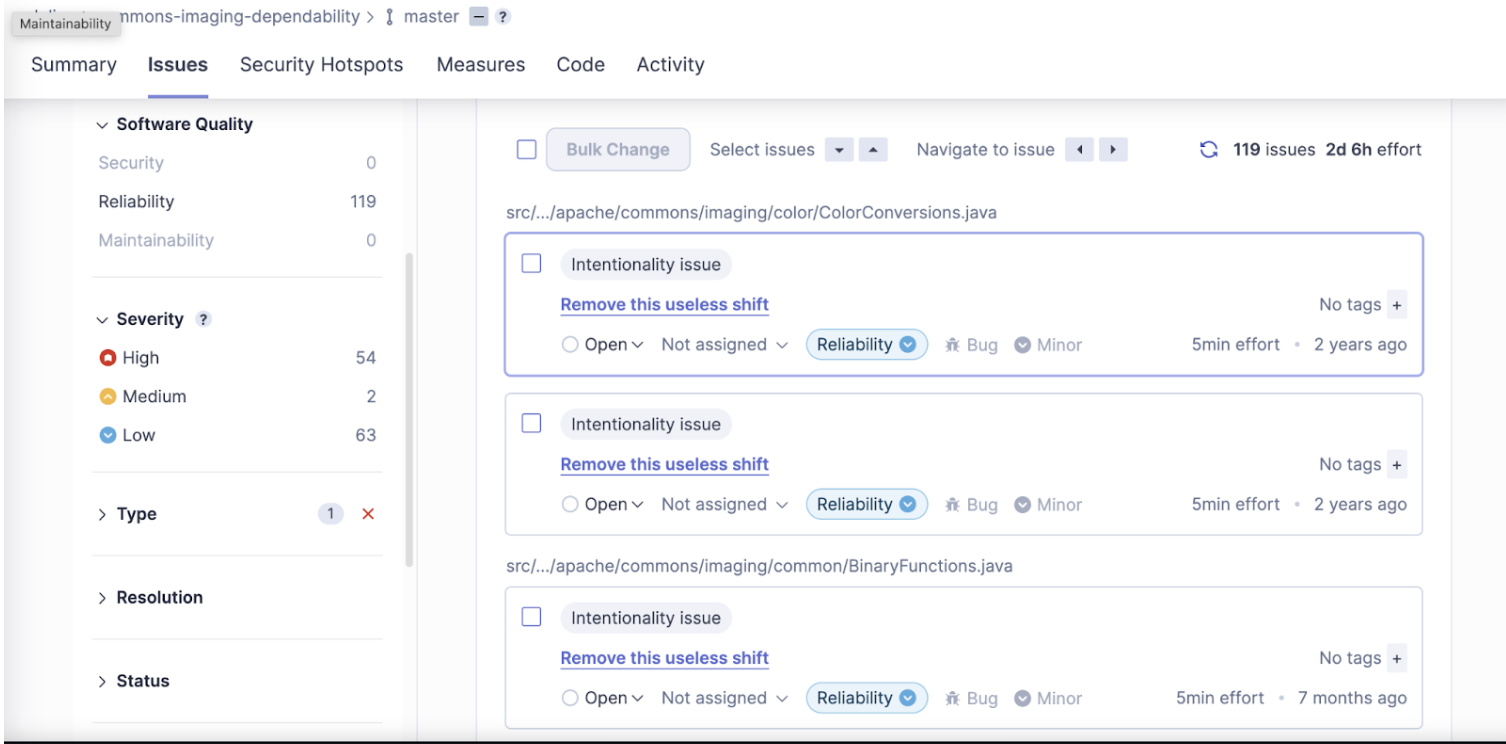
\includegraphics[width=1\linewidth]{reportSonarCloud.png}
    \caption{Report before fix}
    \label{fig:enter-label}
\end{figure}


\subsection{Analyzing SonarCloud}

After analyzing the commons-imaging-dependability project on SonarCloud, we found the following issues in the code:

\textbf{High → 109}

In the high category, several errors are related to divisions where the divisor is not checked for the possibility of being 0. Therefore, if the divisor is 0, the code would throw an exception. There are also errors of the type where referencing a static member of a subclass from its parent during class initialization makes the code more fragile and prone to future errors. The program's execution will largely depend on the order of class and static member initialization.

\textbf{Medium → 2}

In the medium category, there are only 2 errors where an attempt is made to get the length of a palette that could be null.

\textbf{Low → 63}

Out of these 63 errors, most are related to the suggestion to remove a left shift, explaining that an int is a 32-bit variable and specifying that shifting an int by 32 is the same as shifting by 0, and shifting by 33 is the same as shifting by 1. Additionally, there are some errors related to number casting.

\subsection{Bugs Fixed}

To organize our tasks based on the errors found in \textbf{SonarCloud}, we created tasks in \textbf{JIRA}, and each of them was assigned to the three members of the group. We attempted to address the majority of the 119 issues related to reliability, of which we were able to fix XX.

\begin{figure}[h!]
    \centering
    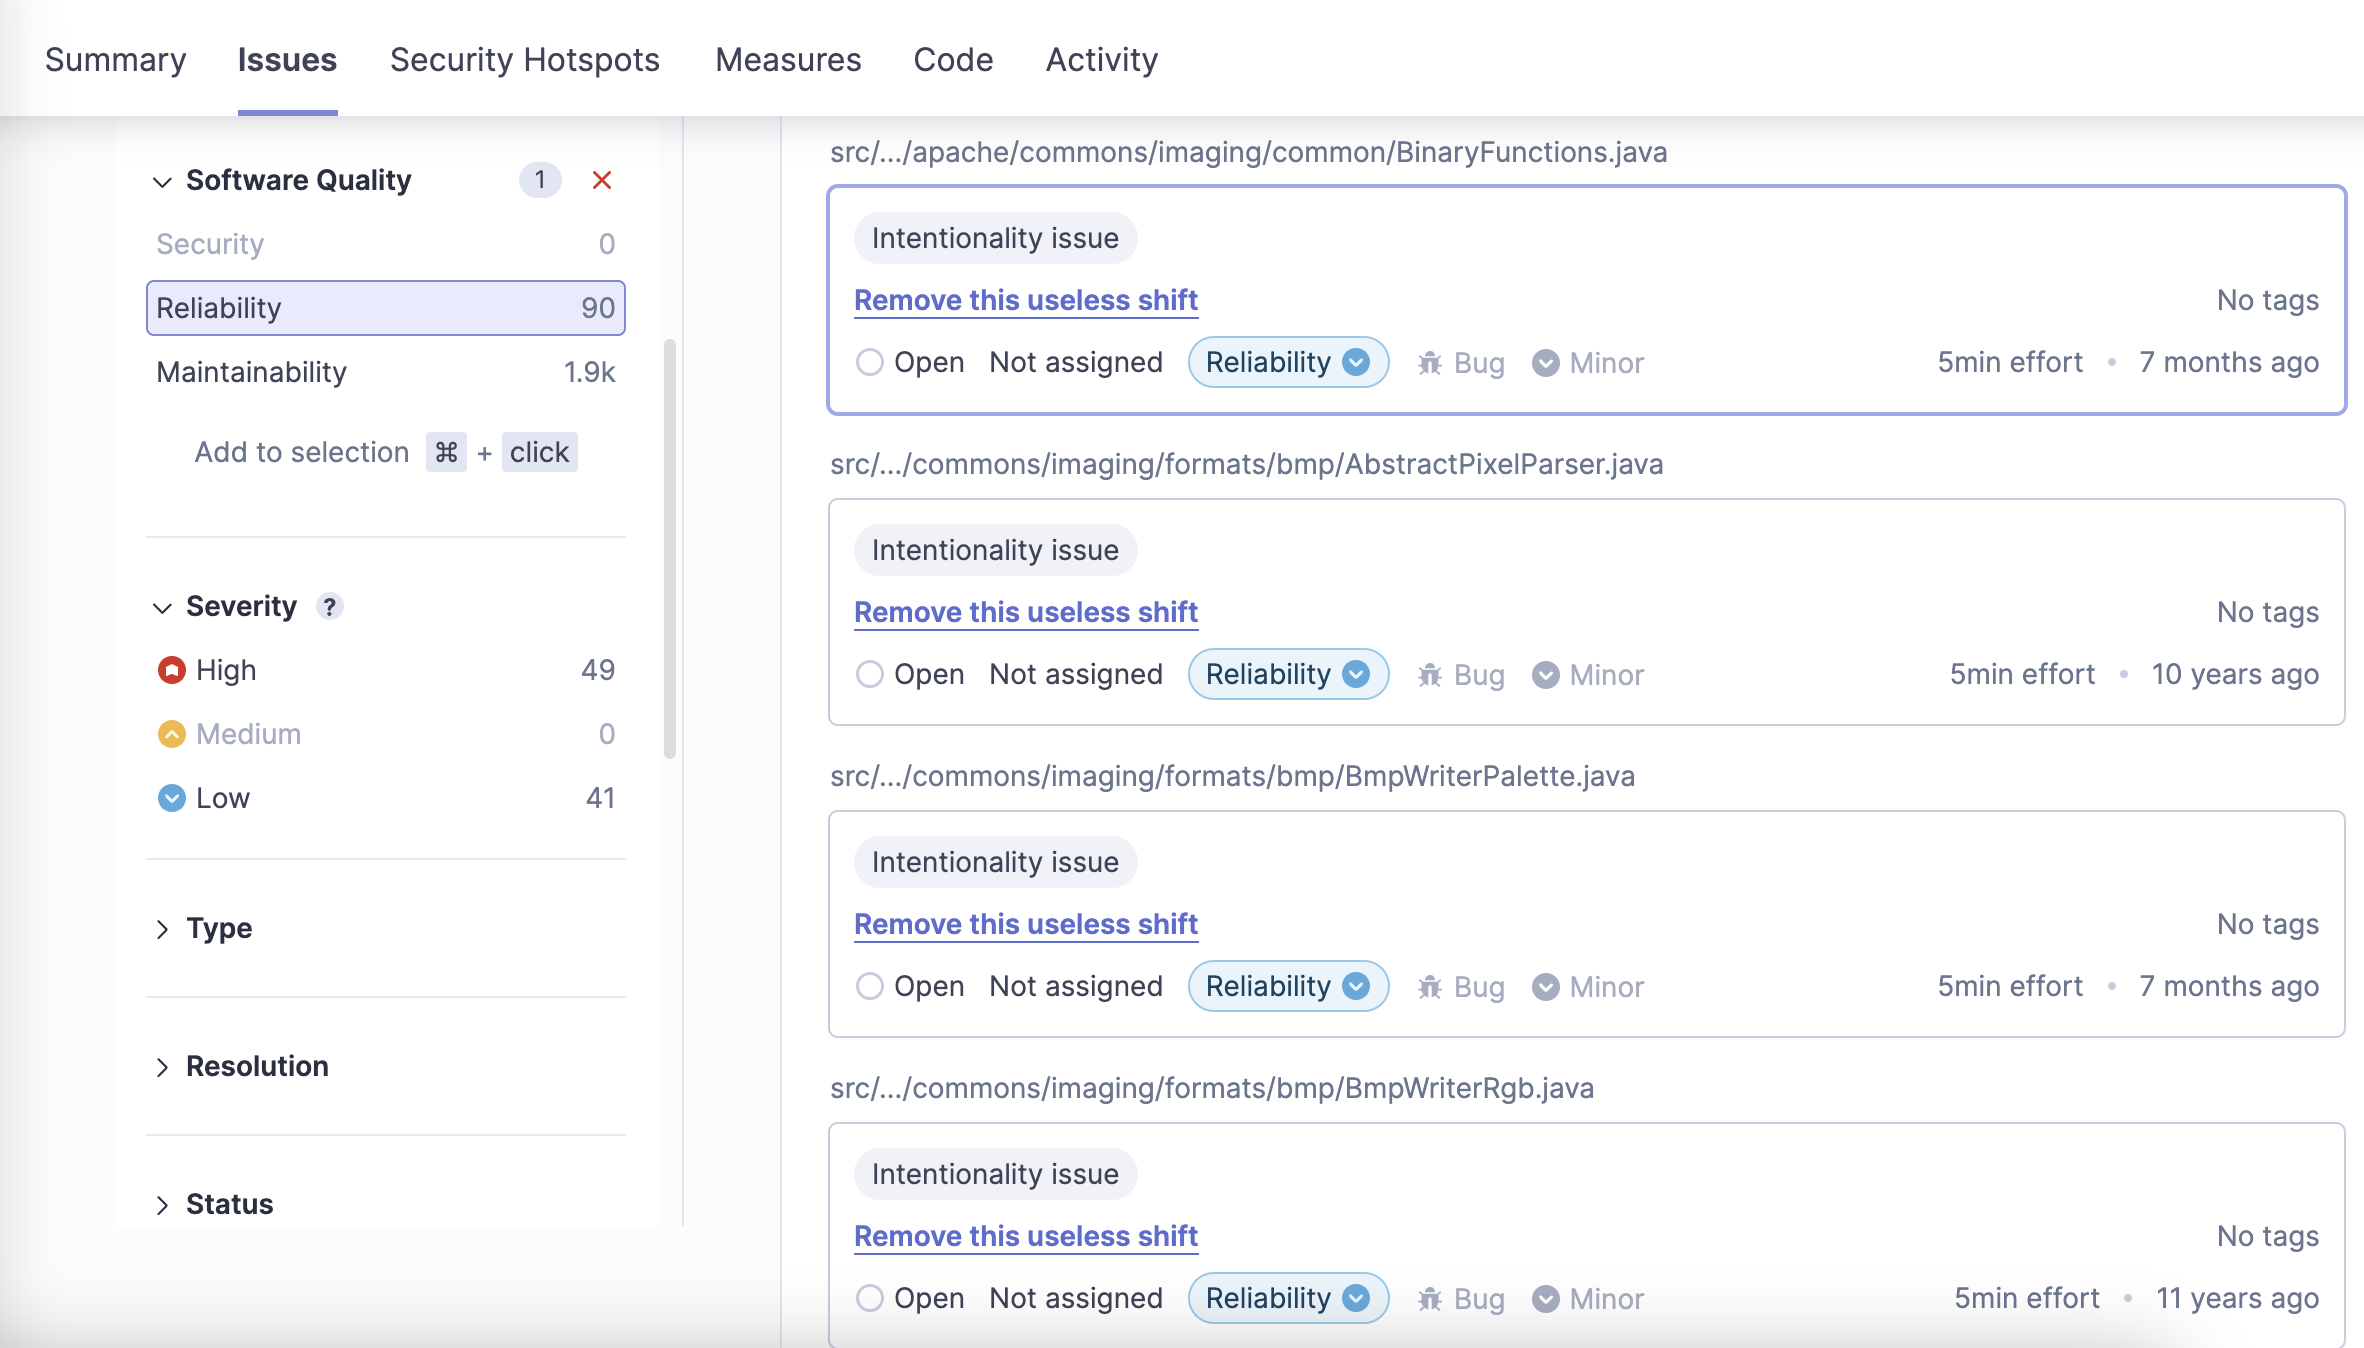
\includegraphics[width=1\linewidth]{reportSonarCloudFixed.png}
    \caption{Bugs Fixed}
    \label{fig:enter-label}
\end{figure}


\section{Title Information}

The title of your work should use capital letters appropriately -
\url{https://capitalizemytitle.com/} has useful rules for
capitalization. Use the {\verb|title|} command to define the title of
your work. If your work has a subtitle, define it with the
{\verb|subtitle|} command.  Do not insert line breaks in your title.

If your title is lengthy, you must define a short version to be used
in the page headers, to prevent overlapping text. The \verb|title|
command has a ``short title'' parameter:
\begin{verbatim}
  \title[short title]{full title}
\end{verbatim}

\section{Authors and Affiliations}

Each author must be defined separately for accurate metadata
identification. Multiple authors may share one affiliation. Authors'
names should not be abbreviated; use full first names wherever
possible. Include authors' e-mail addresses whenever possible.

Grouping authors' names or e-mail addresses, or providing an ``e-mail
alias,'' as shown below, is not acceptable:
\begin{verbatim}
  \author{Brooke Aster, David Mehldau}
  \email{dave,judy,steve@university.edu}
  \email{firstname.lastname@phillips.org}
\end{verbatim}

The \verb|authornote| and \verb|authornotemark| commands allow a note
to apply to multiple authors --- for example, if the first two authors
of an article contributed equally to the work.

If your author list is lengthy, you must define a shortened version of
the list of authors to be used in the page headers, to prevent
overlapping text. The following command should be placed just after
the last \verb|\author{}| definition:
\begin{verbatim}
  \renewcommand{\shortauthors}{McCartney, et al.}
\end{verbatim}
Omitting this command will force the use of a concatenated list of all
of the authors' names, which may result in overlapping text in the
page headers.

The article template's documentation, available at
\url{https://www.acm.org/publications/proceedings-template}, has a
complete explanation of these commands and tips for their effective
use.

Note that authors' addresses are mandatory for journal articles.

\section{Rights Information}

Authors of any work published by ACM will need to complete a rights
form. Depending on the kind of work, and the rights management choice
made by the author, this may be copyright transfer, permission,
license, or an OA (open access) agreement.

Regardless of the rights management choice, the author will receive a
copy of the completed rights form once it has been submitted. This
form contains \LaTeX\ commands that must be copied into the source
document. When the document source is compiled, these commands and
their parameters add formatted text to several areas of the final
document:
\begin{itemize}
\item the ``ACM Reference Format'' text on the first page.
\item the ``rights management'' text on the first page.
\item the conference information in the page header(s).
\end{itemize}

Rights information is unique to the work; if you are preparing several
works for an event, make sure to use the correct set of commands with
each of the works.

The ACM Reference Format text is required for all articles over one
page in length, and is optional for one-page articles (abstracts).

\section{CCS Concepts and User-Defined Keywords}

Two elements of the ``acmart'' document class provide powerful
taxonomic tools for you to help readers find your work in an online
search.

The ACM Computing Classification System ---
\url{https://www.acm.org/publications/class-2012} --- is a set of
classifiers and concepts that describe the computing
discipline. Authors can select entries from this classification
system, via \url{https://dl.acm.org/ccs/ccs.cfm}, and generate the
commands to be included in the \LaTeX\ source.

User-defined keywords are a comma-separated list of words and phrases
of the authors' choosing, providing a more flexible way of describing
the research being presented.

CCS concepts and user-defined keywords are required for for all
articles over two pages in length, and are optional for one- and
two-page articles (or abstracts).

\section{Sectioning Commands}

Your work should use standard \LaTeX\ sectioning commands:
\verb|section|, \verb|subsection|, \verb|subsubsection|, and
\verb|paragraph|. They should be numbered; do not remove the numbering
from the commands.

Simulating a sectioning command by setting the first word or words of
a paragraph in boldface or italicized text is {\bfseries not allowed.}

\section{Tables}

The ``\verb|acmart|'' document class includes the ``\verb|booktabs|''
package --- \url{https://ctan.org/pkg/booktabs} --- for preparing
high-quality tables.

Table captions are placed {\itshape above} the table.

Because tables cannot be split across pages, the best placement for
them is typically the top of the page nearest their initial cite.  To
ensure this proper ``floating'' placement of tables, use the
environment \textbf{table} to enclose the table's contents and the
table caption.  The contents of the table itself must go in the
\textbf{tabular} environment, to be aligned properly in rows and
columns, with the desired horizontal and vertical rules.  Again,
detailed instructions on \textbf{tabular} material are found in the
\textit{\LaTeX\ User's Guide}.

Immediately following this sentence is the point at which
Table~\ref{tab:freq} is included in the input file; compare the
placement of the table here with the table in the printed output of
this document.

\begin{table}
  \caption{Frequency of Special Characters}
  \label{tab:freq}
  \begin{tabular}{ccl}
    \toprule
    Non-English or Math&Frequency&Comments\\
    \midrule
    \O & 1 in 1,000& For Swedish names\\
    $\pi$ & 1 in 5& Common in math\\
    \$ & 4 in 5 & Used in business\\
    $\Psi^2_1$ & 1 in 40,000& Unexplained usage\\
  \bottomrule
\end{tabular}
\end{table}

To set a wider table, which takes up the whole width of the page's
live area, use the environment \textbf{table*} to enclose the table's
contents and the table caption.  As with a single-column table, this
wide table will ``float'' to a location deemed more
desirable. Immediately following this sentence is the point at which
Table~\ref{tab:commands} is included in the input file; again, it is
instructive to compare the placement of the table here with the table
in the printed output of this document.

\begin{table*}
  \caption{Some Typical Commands}
  \label{tab:commands}
  \begin{tabular}{ccl}
    \toprule
    Command &A Number & Comments\\
    \midrule
    \texttt{{\char'134}author} & 100& Author \\
    \texttt{{\char'134}table}& 300 & For tables\\
    \texttt{{\char'134}table*}& 400& For wider tables\\
    \bottomrule
  \end{tabular}
\end{table*}

Always use midrule to separate table header rows from data rows, and
use it only for this purpose. This enables assistive technologies to
recognise table headers and support their users in navigating tables
more easily.

\section{Math Equations}
You may want to display math equations in three distinct styles:
inline, numbered or non-numbered display.  Each of the three are
discussed in the next sections.

\subsection{Inline (In-text) Equations}
A formula that appears in the running text is called an inline or
in-text formula.  It is produced by the \textbf{math} environment,
which can be invoked with the usual
\texttt{{\char'134}begin\,\ldots{\char'134}end} construction or with
the short form \texttt{\$\,\ldots\$}. You can use any of the symbols
and structures, from $\alpha$ to $\omega$, available in
\LaTeX~\cite{Lamport:LaTeX}; this section will simply show a few
examples of in-text equations in context. Notice how this equation:
\begin{math}
  \lim_{n\rightarrow \infty}x=0
\end{math},
set here in in-line math style, looks slightly different when
set in display style.  (See next section).

\subsection{Display Equations}
A numbered display equation---one set off by vertical space from the
text and centered horizontally---is produced by the \textbf{equation}
environment. An unnumbered display equation is produced by the
\textbf{displaymath} environment.

Again, in either environment, you can use any of the symbols and
structures available in \LaTeX\@; this section will just give a couple
of examples of display equations in context.  First, consider the
equation, shown as an inline equation above:
\begin{equation}
  \lim_{n\rightarrow \infty}x=0
\end{equation}
Notice how it is formatted somewhat differently in
the \textbf{displaymath}
environment.  Now, we'll enter an unnumbered equation:
\begin{displaymath}
  \sum_{i=0}^{\infty} x + 1
\end{displaymath}
and follow it with another numbered equation:
\begin{equation}
  \sum_{i=0}^{\infty}x_i=\int_{0}^{\pi+2} f
\end{equation}
just to demonstrate \LaTeX's able handling of numbering.

\section{Figures}

The ``\verb|figure|'' environment should be used for figures. One or
more images can be placed within a figure. If your figure contains
third-party material, you must clearly identify it as such, as shown
in the example below.
\begin{figure}[h]
  \centering
  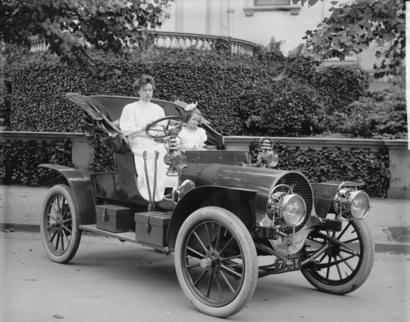
\includegraphics[width=\linewidth]{sample-franklin}
  \caption{1907 Franklin Model D roadster. Photograph by Harris \&
    Ewing, Inc. [Public domain], via Wikimedia
    Commons. (\url{https://goo.gl/VLCRBB}).}
  \Description{A woman and a girl in white dresses sit in an open car.}
\end{figure}

Your figures should contain a caption which describes the figure to
the reader.

Figure captions are placed {\itshape below} the figure.

Every figure should also have a figure description unless it is purely
decorative. These descriptions convey what’s in the image to someone
who cannot see it. They are also used by search engine crawlers for
indexing images, and when images cannot be loaded.

A figure description must be unformatted plain text less than 2000
characters long (including spaces).  {\bfseries Figure descriptions
  should not repeat the figure caption – their purpose is to capture
  important information that is not already provided in the caption or
  the main text of the paper.} For figures that convey important and
complex new information, a short text description may not be
adequate. More complex alternative descriptions can be placed in an
appendix and referenced in a short figure description. For example,
provide a data table capturing the information in a bar chart, or a
structured list representing a graph.  For additional information
regarding how best to write figure descriptions and why doing this is
so important, please see
\url{https://www.acm.org/publications/taps/describing-figures/}.

\subsection{The ``Teaser Figure''}

A ``teaser figure'' is an image, or set of images in one figure, that
are placed after all author and affiliation information, and before
the body of the article, spanning the page. If you wish to have such a
figure in your article, place the command immediately before the
\verb|\maketitle| command:
\begin{verbatim}
  \begin{teaserfigure}
    \includegraphics[width=\textwidth]{sampleteaser}
    \caption{figure caption}
    \Description{figure description}
  \end{teaserfigure}
\end{verbatim}

\section{Citations and Bibliographies}

The use of \BibTeX\ for the preparation and formatting of one's
references is strongly recommended. Authors' names should be complete
--- use full first names (``Donald E. Knuth'') not initials
(``D. E. Knuth'') --- and the salient identifying features of a
reference should be included: title, year, volume, number, pages,
article DOI, etc.

The bibliography is included in your source document with these two
commands, placed just before the \verb|\end{document}| command:
\begin{verbatim}
  \bibliographystyle{ACM-Reference-Format}
  \bibliography{bibfile}
\end{verbatim}
where ``\verb|bibfile|'' is the name, without the ``\verb|.bib|''
suffix, of the \BibTeX\ file.

Citations and references are numbered by default. A small number of
ACM publications have citations and references formatted in the
``author year'' style; for these exceptions, please include this
command in the {\bfseries preamble} (before the command
``\verb|\begin{document}|'') of your \LaTeX\ source:
\begin{verbatim}
  \citestyle{acmauthoryear}
\end{verbatim}

  Some examples.  A paginated journal article \cite{Abril07}, an
  enumerated journal article \cite{Cohen07}, a reference to an entire
  issue \cite{JCohen96}, a monograph (whole book) \cite{Kosiur01}, a
  monograph/whole book in a series (see 2a in spec. document)
  \cite{Harel79}, a divisible-book such as an anthology or compilation
  \cite{Editor00} followed by the same example, however we only output
  the series if the volume number is given \cite{Editor00a} (so
  Editor00a's series should NOT be present since it has no vol. no.),
  a chapter in a divisible book \cite{Spector90}, a chapter in a
  divisible book in a series \cite{Douglass98}, a multi-volume work as
  book \cite{Knuth97}, a couple of articles in a proceedings (of a
  conference, symposium, workshop for example) (paginated proceedings
  article) \cite{Andler79, Hagerup1993}, a proceedings article with
  all possible elements \cite{Smith10}, an example of an enumerated
  proceedings article \cite{VanGundy07}, an informally published work
  \cite{Harel78}, a couple of preprints \cite{Bornmann2019,
    AnzarootPBM14}, a doctoral dissertation \cite{Clarkson85}, a
  master's thesis: \cite{anisi03}, an online document / world wide web
  resource \cite{Thornburg01, Ablamowicz07, Poker06}, a video game
  (Case 1) \cite{Obama08} and (Case 2) \cite{Novak03} and \cite{Lee05}
  and (Case 3) a patent \cite{JoeScientist001}, work accepted for
  publication \cite{rous08}, 'YYYYb'-test for prolific author
  \cite{SaeediMEJ10} and \cite{SaeediJETC10}. Other cites might
  contain 'duplicate' DOI and URLs (some SIAM articles)
  \cite{Kirschmer:2010:AEI:1958016.1958018}. Boris / Barbara Beeton:
  multi-volume works as books \cite{MR781536} and \cite{MR781537}. A
  couple of citations with DOIs:
  \cite{2004:ITE:1009386.1010128,Kirschmer:2010:AEI:1958016.1958018}. Online
  citations: \cite{TUGInstmem, Thornburg01, CTANacmart}. Artifacts:
  \cite{R} and \cite{UMassCitations}.

\section{Acknowledgments}

Identification of funding sources and other support, and thanks to
individuals and groups that assisted in the research and the
preparation of the work should be included in an acknowledgment
section, which is placed just before the reference section in your
document.

This section has a special environment:
\begin{verbatim}
  \begin{acks}
  ...
  \end{acks}
\end{verbatim}
so that the information contained therein can be more easily collected
during the article metadata extraction phase, and to ensure
consistency in the spelling of the section heading.

Authors should not prepare this section as a numbered or unnumbered {\verb|\section|}; please use the ``{\verb|acks|}'' environment.

\section{Appendices}

If your work needs an appendix, add it before the
``\verb|\end{document}|'' command at the conclusion of your source
document.

Start the appendix with the ``\verb|appendix|'' command:
\begin{verbatim}
  \appendix
\end{verbatim}
and note that in the appendix, sections are lettered, not
numbered. This document has two appendices, demonstrating the section
and subsection identification method.

\section{Multi-language papers}

Papers may be written in languages other than English or include
titles, subtitles, keywords and abstracts in different languages (as a
rule, a paper in a language other than English should include an
English title and an English abstract).  Use \verb|language=...| for
every language used in the paper.  The last language indicated is the
main language of the paper.  For example, a French paper with
additional titles and abstracts in English and German may start with
the following command
\begin{verbatim}
\documentclass[sigconf, language=english, language=german,
               language=french]{acmart}
\end{verbatim}

The title, subtitle, keywords and abstract will be typeset in the main
language of the paper.  The commands \verb|\translatedXXX|, \verb|XXX|
begin title, subtitle and keywords, can be used to set these elements
in the other languages.  The environment \verb|translatedabstract| is
used to set the translation of the abstract.  These commands and
environment have a mandatory first argument: the language of the
second argument.  See \verb|sample-sigconf-i13n.tex| file for examples
of their usage.

\section{SIGCHI Extended Abstracts}

The ``\verb|sigchi-a|'' template style (available only in \LaTeX\ and
not in Word) produces a landscape-orientation formatted article, with
a wide left margin. Three environments are available for use with the
``\verb|sigchi-a|'' template style, and produce formatted output in
the margin:
\begin{itemize}
\item {\verb|sidebar|}:  Place formatted text in the margin.
\item {\verb|marginfigure|}: Place a figure in the margin.
\item {\verb|margintable|}: Place a table in the margin.
\end{itemize}

%%
%% The acknowledgments section is defined using the "acks" environment
%% (and NOT an unnumbered section). This ensures the proper
%% identification of the section in the article metadata, and the
%% consistent spelling of the heading.
\begin{acks}
To Robert, for the bagels and explaining CMYK and color spaces.
\end{acks}

%%
%% The next two lines define the bibliography style to be used, and
%% the bibliography file.
\bibliographystyle{ACM-Reference-Format}
\bibliography{sample-base}

%%
%% If your work has an appendix, this is the place to put it.
\appendix

\section{Research Methods}

\subsection{Part One}

Lorem ipsum dolor sit amet, consectetur adipiscing elit. Morbi
malesuada, quam in pulvinar varius, metus nunc fermentum urna, id
sollicitudin purus odio sit amet enim. Aliquam ullamcorper eu ipsum
vel mollis. Curabitur quis dictum nisl. Phasellus vel semper risus, et
lacinia dolor. Integer ultricies commodo sem nec semper.

\subsection{Part Two}

Etiam commodo feugiat nisl pulvinar pellentesque. Etiam auctor sodales
ligula, non varius nibh pulvinar semper. Suspendisse nec lectus non
ipsum convallis congue hendrerit vitae sapien. Donec at laoreet
eros. Vivamus non purus placerat, scelerisque diam eu, cursus
ante. Etiam aliquam tortor auctor efficitur mattis.

\section{Online Resources}

Nam id fermentum dui. Suspendisse sagittis tortor a nulla mollis, in
pulvinar ex pretium. Sed interdum orci quis metus euismod, et sagittis
enim maximus. Vestibulum gravida massa ut felis suscipit
congue. Quisque mattis elit a risus ultrices commodo venenatis eget
dui. Etiam sagittis eleifend elementum.

Nam interdum magna at lectus dignissim, ac dignissim lorem
rhoncus. Maecenas eu arcu ac neque placerat aliquam. Nunc pulvinar
massa et mattis lacinia.

\end{document}